\textbf{COLUNI 2019 -- Questão 25}\par\medskip Em uma amostra natural de um elemento químico, os átomos desse elemento têm, na maioria das vezes, massas diferentes. Muitos desses elementos químicos têm, pelo menos, dois isótopos estáveis (não radioativos), mas alguns (por exemplo, o alumínio) têm somente um, e outros (por exemplo, o estanho) têm muitos isótopos.

\par

Observe o gráfico a seguir, que apresenta as massas dos isótopos de cinco elementos químicos:

% COLUNI-AUTO-FIGURES-BEGIN
\begin{figure}[htbp]
\centering
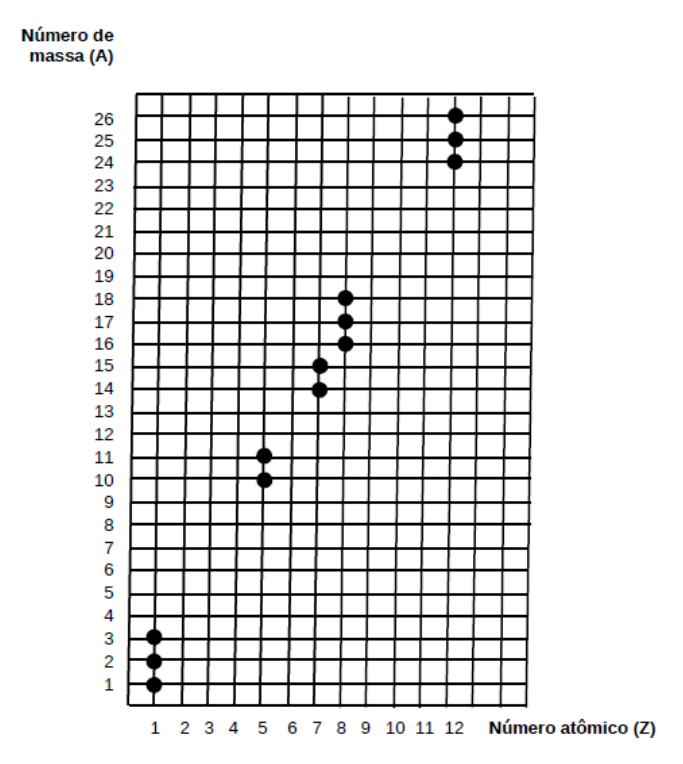
\includegraphics[width=0.95\linewidth]{static/simulados/coluni/figuras/2019/questao-25/figura-1.png}
\end{figure}
% COLUNI-AUTO-FIGURES-END

Com base nas informações fornecidas e nos conhecimentos sobre ciências, assinale a afirmativa CORRETA:


\begin{enumerate}
\item O elemento nitrogênio tem dois isótopos cujos átomos diferem por apresentarem 14 ou 15 nêutrons.
\item As espécies químicas $^{18}\mathrm{O}$ e $^{26}\mathrm{Mg}$ têm o mesmo excesso de nêutrons em relação ao número de prótons.
\item Os átomos isótopos neutros do elemento oxigênio diferem entre si quanto ao número de elétrons.
\item O cátion monovalente do elemento oxigênio e o cátion bivalente do elemento magnésio são isoeletrônicos.\end{enumerate}
